\documentclass[a4paper,12pt]{article}
\linespread{1.3} % 1.5 interval 
\usepackage[left=2cm, right=1.5cm, top=3cm, bottom=3cm]{geometry} % Page size
\usepackage[colorlinks]{hyperref} % Colors for hypersmth
\hypersetup{
    colorlinks = true,
    linkcolor= black, % black color for table of contents
    citecolor= black
   }
\usepackage{graphicx} % Required for inserting images
\usepackage{listings} % Code
\usepackage[compact]{titlesec} % Table of contents
\usepackage{indentfirst} % Indent at each paragraph
\setcounter{page}{-1} % Start from zero
\usepackage{amsmath,float} % Everyone needs it, don't lie
%\numberwithin{figure}{section} % Figures are numbered with the section number
\usepackage[dvipsnames,table,xcdraw]{xcolor} % Allow colors in the documents
\usepackage{bashful} % Write a code
%\usepackage{subfigure} % Put two fig side by side
\usepackage{subfig} % Another variant of this
\usepackage{comment} % comment out large sections
\usepackage{datetime} % Use for reading dates
\usepackage{multirow} % for tables
\usepackage{longtable} % long tables
\newcolumntype{C}[1]{>{\centering\arraybackslash}p{#1}} 
\usepackage{array}

\usepackage{tikz}
\usepackage{eso-pic}
%\usepackage{blindtext}

\newsavebox\logoone
\sbox\logoone{
  \tikz[overlay]
  \node[anchor=north east, inner sep=20pt] at (current page.north east){%
    
\includegraphics[scale=0.3]{BrandIcon.png}};}


\setcounter{secnumdepth}{1}

\titleformat{\paragraph}
{\normalfont\normalsize\bfseries}{\theparagraph}{1em}{}
\titlespacing*{\paragraph}
{0pt}{3.25ex plus 1ex minus .2ex}{1.5ex plus .2ex}

\newdateformat{monthyeardate}{%
  \monthname[\THEMONTH], \THEYEAR}

\usepackage{nameref} % Reference by name
\newcommand*{\secref}[1]{\textbf{\hyperref[{#1}]{\nameref*{#1} Section \ref*{#1}}}}
%% The cleveref is the last
\usepackage{enumitem}
\usepackage[norsk,nameinlink,capitalize]{cleveref} % Short and capitalized cross-references
%% Format for equations citation
\crefrangeformat{equation}{Eqs.~#3#1#4 to~#5#2#6}
\crefrangeformat{figure}{Figs.~#3#1#4 to~#5#2#6}
\crefformat{equation}{Eq.~#2#1#3}
\crefformat{figure}{Fig.~#2#1#3}
\Crefformat{figure}{Figure~#2#1#3}
\crefformat{table}{Table~#2#1#3}
\crefformat{section}{Section~#2#1#3}


\begin{document}
% Begin the title page
\thispagestyle{empty}

\includegraphics[width=0.5\textwidth]{Logo.pdf}

\vspace{8cm}

\begin{center}
{\huge\textbf{Japanese society for \\
food science and technology}}
\end{center}
\vspace{1cm}


{\LARGE
Sample Preparation and Application Use

\vspace{1cm}

For SANYO Trading
}
\vfill

%\monthyeardate\today  
\today


% End of the title page


% Begin Table of contents
\newpage
\thispagestyle{empty}
\AddToShipoutPictureBG{\usebox\logoone}
\tableofcontents


\newpage
\section{Sample Preparation}
\label{sec:Samples}

This section explains how the samples are prepared and provides examples of parameter calculations. 

\textbf{A total of 16 NMR ampules are required: 15 for the samples and 1 for the Glycerol Standard. Precise balances are used during preparation.}

These samples will be used for calibration and later for demonstrations. 
Different measurement parameters are available for each sample type and are listed in the corresponding sections. 
Calibration sets are made by mixing two original food products and weighing their masses ($Mass_1$ and $Mass_2$). 
With the known content of X (such as Carbohydrates, Oils, Fats, etc.) in the pure products ($Content_1$ and $Content_2$), the content of X in the mixture ($Content_m$) can be calculated as:

\begin{equation}
    Content_m = 100 \cdot \frac{Mass_1 \cdot Content_1 + Mass_2 \cdot Content_2}{Mass_1 + Mass_2}
\end{equation}

\subsection{Milk Powder}
\label{sec:Milk Powder}
Several parameters are available for measurement in the mixtures of milk powder:
\begin{enumerate}
    \item Protein Content
    \item Fat Content
    \item Carbohydrates content
\end{enumerate}

To prepare calibration set for Milk Powder we took two different products with known contents of Proteins, Carbohydrates (C.H.) and Fats as shown in \cref{tab:Milk Pure}  and mixed them in different proportions. The resulting Fat, Proteins and C.H. contents are given in \cref{tab:Milk Mixture} below.
The Samples 1 and 5 are pure products, whereas 2, 3 and 4 are mixtures.

\begin{table}[ht!]
\centering
\caption{The contents in pure milk powder products}
\label{tab:Milk Pure}
\begin{tabular}{|c|c|c|}
\hline
Content   X   & Powder 1 & Powder 2 \\ \hline
Protein       & 1.7\%     & 35.5\%     \\ \hline
Carbohydrates & 57.1\%     & 51.7\%   \\ \hline
Fat           & 35.0\%     & 1.0\%   \\ \hline
\end{tabular}
\end{table}

\textbf{The key recommendation for preparing these samples is to ensure thorough mixing. It is important to avoid using large masses; aim to keep the mass close to 0.3 grams or less. Make sure the resulting mixture is evenly distributed in the ampule.
}

\begin{table}[H]
\centering
\caption{The contents in mixtures of milk powders}
\label{tab:Milk Mixture}
\begin{tabular}{|c|c|c|c|}
\hline
\textbf{\# Sample} & \textbf{$\omega$\% Fat} & \textbf{$\omega$\% Proteins} & \textbf{$\omega$\% C.H.} \\ \hline
1                  & 35.0             & 57.1                  & 1.7               \\ \hline
2                  & 15.3             & 54.0                  & 21.3              \\ \hline
3                  & 10.1             & 53.1                  & 26.4              \\ \hline
4                  & 4.7              & 52.3                  & 31.9              \\ \hline
5                  & 1.0              & 51.7                  & 35.5              \\ \hline
\end{tabular}
\end{table}

The example of calculation of Fat content for the Sample 2 is given below. To prepare this sample $0.1016$ g of milk powder with $35$\% fat was taken and $0.1397$ g of milk powder with $1$\% fat:

\begin{equation}
    \omega(Fat)_2 = 100 \cdot \frac{0.1016 \cdot 0.35 + 0.1397 \cdot 0.01}{0.1016 + 0.1397} = 15.3\%
\end{equation}

\begin{figure}[H]
\centering
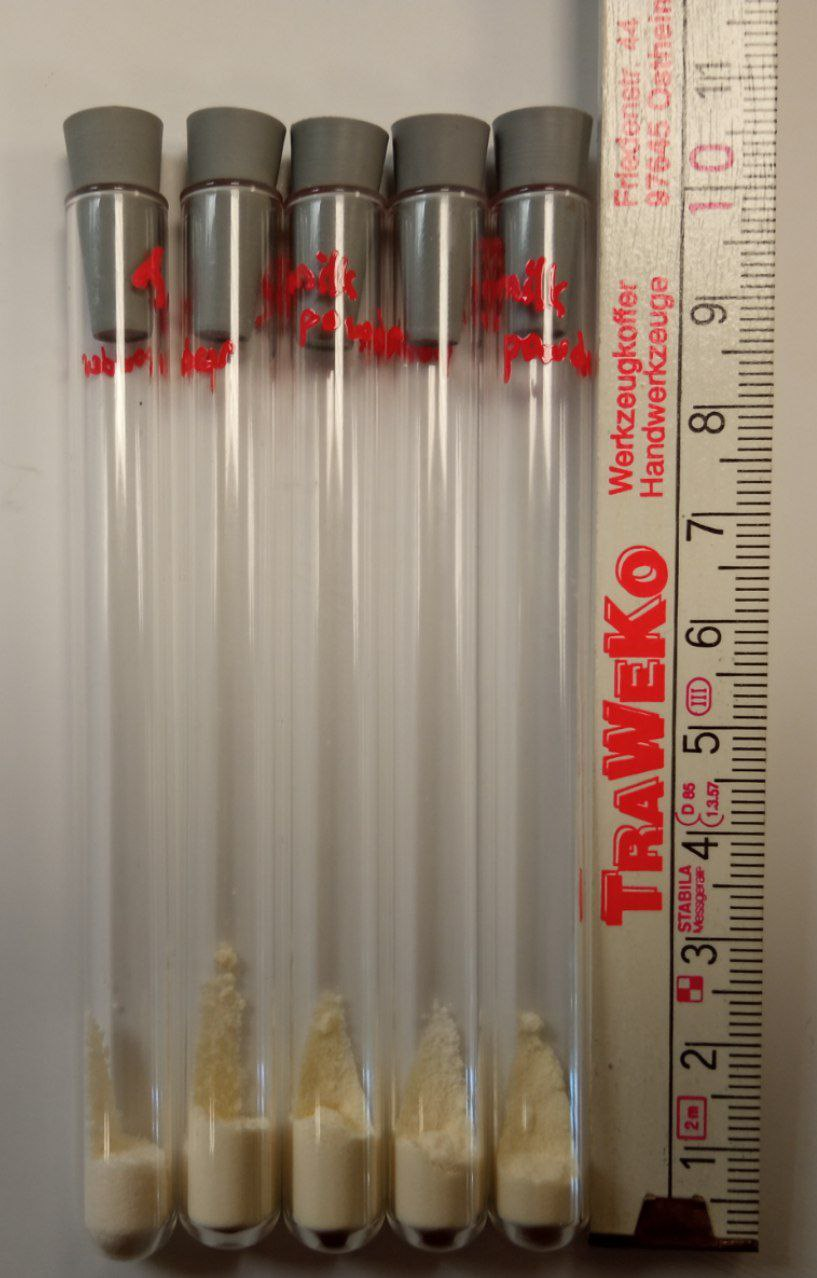
\includegraphics[width=5cm]{milk.jpg}
\caption{Ready for measurement samples with milk powder}
\label{fig:milk}
\end{figure}

\subsection{Cookies}
\label{sec:Cookies}

Several parameters are available for measurement in the cookies:
\begin{enumerate}
    \item Fat Content
    \item Carbohydrates content
\end{enumerate}

To prepare calibration set for Cookies we took two different products with known contents of Carbohydrates (C.H.) and Fats as shown in \cref{tab:Cookies Pure}  and mixed them in different proportions. 
The resulting Fat and C.H. contents are given in \cref{tab:Cookies Mixture} below.
The Samples 1 and 5 are pure products, whereas 2, 3 and 4 are mixtures.

\begin{table}[ht!]
\centering
\caption{The contents in pure cookies}
\label{tab:Cookies Pure}
\begin{tabular}{|c|c|c|}
\hline
Content   X   & Cookie 1 & Cookie 2 \\ \hline
Carbohydrates & 70\%      & 80\%      \\ \hline
Fat           & 14\%      & 7\%       \\ \hline
\end{tabular}
\end{table}

\textbf{
Use a mortar and pestle, or a similar tool, to grind the solid cookies into fine powders.
The key recommendation for preparing these samples is to ensure thorough mixing. 
It is important to avoid using large masses; aim to keep the mass close to 0.3 grams or less. 
Make sure the resulting mixture is evenly distributed in the ampule.
}

\begin{table}[H]
\centering
\caption{The contents in mixtures of milk powders}
\label{tab:Cookies Mixture}
\begin{tabular}{|c|c|c|}
\hline
\textbf{\#  Sample} & \textbf{$\omega$\% Fat} & \textbf{$\omega$\% C.H.} \\ \hline
1                   & 14.00            & 70.00             \\ \hline
2                   & 11.49            & 73.58             \\ \hline
3                   & 10.45            & 75.08             \\ \hline
4                   & 8.62             & 77.68             \\ \hline
5                   & 7.00             & 80.00             \\ \hline
\end{tabular}
\end{table}

\begin{figure}[H]
\centering
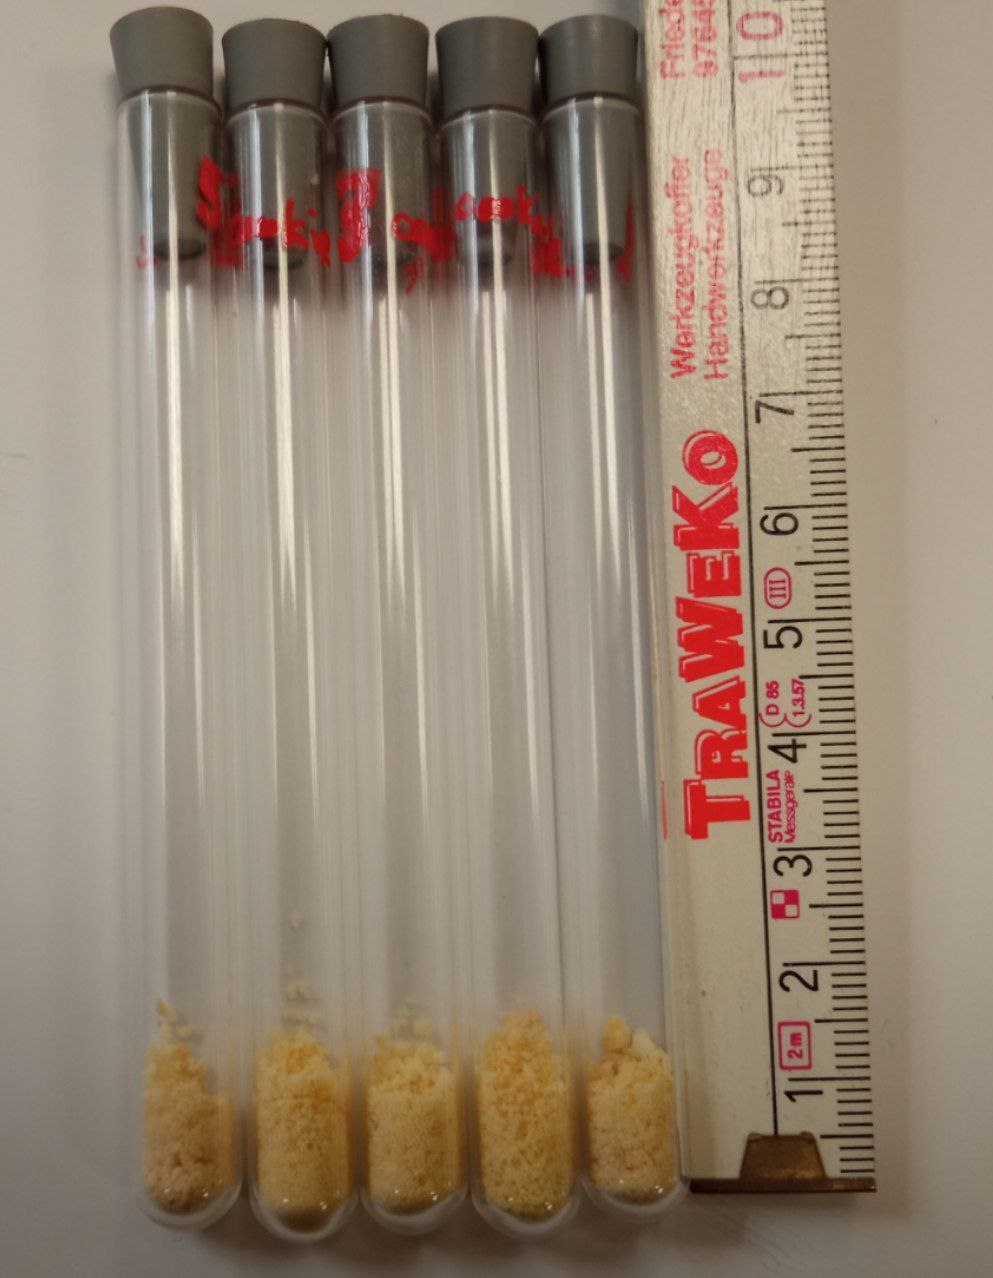
\includegraphics[width=5cm]{cookie.jpg}
\caption{Ready for measurement samples with cookies}
\label{fig:cookie}
\end{figure}

\newpage
\subsection{Butter}
\label{sec:Butter}
The Fat Content parameter is available for measurement in these types of samples.

Two butter products were used to prepare the calibration set. In the first product the fat content is known to be 99.8\%, whereas in the second 82\%.

By mixing them together the samples with the following fat contents were prepared:
\begin{table}[H]
\centering
\caption{The Fat content in mixtures of butter}
\label{tab:Butter Mixture}
\begin{tabular}{|c|c|}
\hline
\textbf{\#  Sample} & \textbf{$\omega$\% Fat} \\ \hline
1                   & 99.80            \\ \hline
2                   & 93.41            \\ \hline
3                   & 91.32            \\ \hline
4                   & 89.62            \\ \hline
5                   & 82.00            \\ \hline
\end{tabular}
\end{table}

\textbf{
Butter melts at relatively low temperatures, typically around 32-34°C. To maintain the consistency of the mixtures, ensure that both the room and storage temperatures remain below the melting point. The samples should be thoroughly mixed to achieve even distribution and homogeneity in the calibration sample.
}

\begin{figure}[H]
\centering
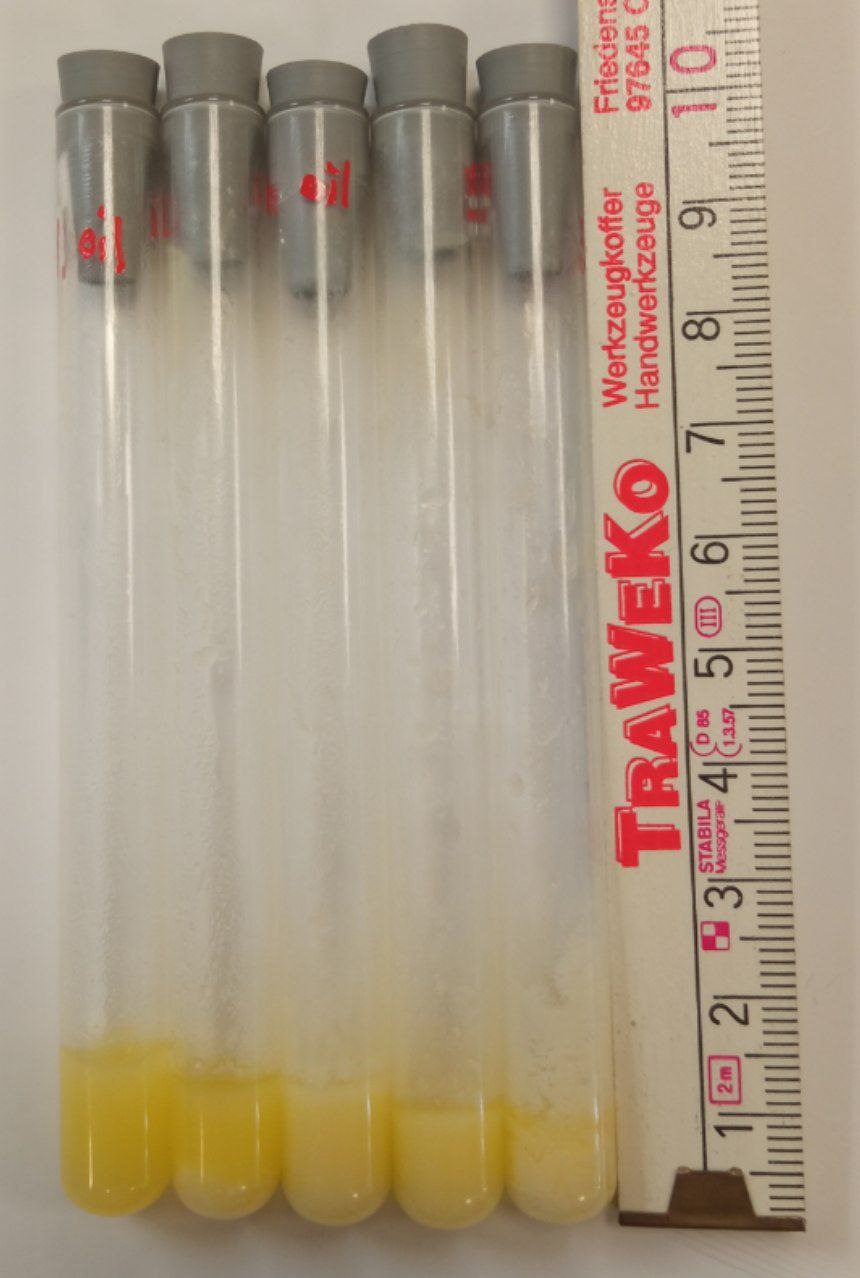
\includegraphics[width=5cm]{butter.jpg}
\caption{Ready for measurement samples with butter}
\label{fig:butter}
\end{figure}

\newpage
\section{Automated hardware tuning}
\label{sec:Automated hardware tuning}

\textbf{The \texttt{Daily Check} application should be run before performing any measurements or calibrations. Running it once is sufficient. After saving the probe, it can be imported into other applications for measurement and calibration.}

\begin{enumerate}
\item Press the Load application and Settings button 
\includegraphics[height=0.5cm]{Btn_Open.png} in the main menu to open the \texttt{Daily Check} application file. The name of the application can be slightly different.

\item Click the Run button 
\includegraphics[height=1cm]{Btn_Start.jpg} to launch the application.

\item The necessary hardware tunings will be performed automatically.

\item Wait for the end of procedure. The Report completed message will appear on the top.

\begin{figure}[H]
\centering

\includegraphics[width=6cm]{Report_Completed.png}
\caption{The \texttt{Daily Check} application successfully finished hardware tuning}
\label{fig:Report_Completed}
\end{figure}

\item To save the applied changes, press the Export Probe button 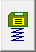
\includegraphics[width=0.7cm]{Settings_Export.png} in the Hardware Tab of Settings window 
\includegraphics[width=0.7cm]{Btn_Settings.png}.

\begin{figure}[!ht]
\centering
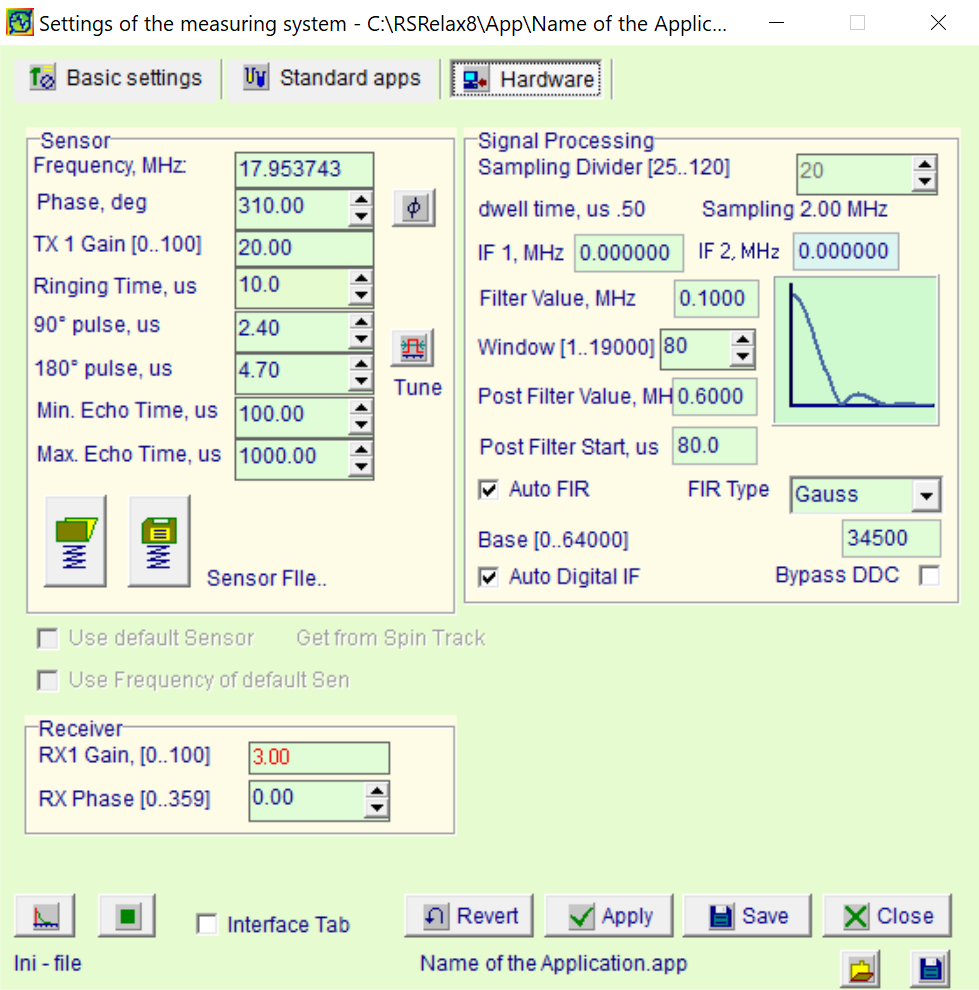
\includegraphics[width=8cm]{Settings_Hardware.png}
\caption{Hardware window}
\label{fig:Hardware window}
\end{figure}
\end{enumerate}

\newpage
\section{Calibration}
\label{sec:Calibration}

The calibration procedure needs to be performed only once before measurement, but after hardware tuning. 
Follow the steps below for each application.
The the step-by-step example on the calibration procedure is given once.
In the following sections only the resulting calibration curves and essential parameters are mentioned.

\begin{enumerate}

\item Press the Load application and Settings button 
\includegraphics[height=0.5cm]{Btn_Open.png} in the main menu to open the corresponding application file.

\item Import the last data from hardware tuning by clicking Import probe button 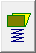
\includegraphics[width=0.7cm]{Settings_Import.png} in the Hardware Window (\cref{fig:Hardware window}).

\item When the Save button 
\includegraphics[height=0.5cm]{Settings_Ini_Save.png} is pressed, the application saves the updated probe parameters. \textbf{This eliminates the need for further hardware tuning for the particular application that day.} In other words, if the application is closed and reopened, or if the operation mode is changed during the day, hardware tuning does not need to be redone.

\item Switch the operation mode to Calibrate. 

\begin{figure}[!ht]
\centering
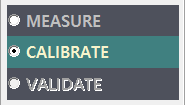
\includegraphics[width=4cm]{Calibrate_Switch.png}
\caption{Switch to Calibrate mode}
\label{fig:Calibrate_mode_switcher}
\end{figure}

\item The calibration tab with calibration table will open.

\item Fill in the following table column cells. Press the Apply button after each cell change:
    \begin{itemize}
        \item Column ID by sample labels (use 1-9 or A-Z with special symbols like $-,_,\%$, if needed).
        \item Column Value by known Content X of the sample.
    \end{itemize}


\item Ensure that values in Settings window are the same as in corresponding figures 

\begin{itemize}
    \item Milk Powders:

Check the values of 
\texttt{Echo times},
\texttt{Relaxation period},
\texttt{Amount of scans},\\
as given in :
\cref{fig:Settings for protein content in milk powders application} and \cref{fig:Gui Settings for protein content in milk powders application}

    \item Cookies:
    
Check the values of 
\texttt{Echo times},
\texttt{Relaxation period} and
\texttt{Amount of scans},\\
as given in :
\cref{fig:Settings for protein content in milk powders application} and \cref{fig:Gui Settings for protein content in milk powders application}    
    
\end{itemize}
Milk powders and Cookies the  are 

are as given in the \cref{fig:Settings for protein content in milk powders application} and \cref{fig:Gui Settings for protein content in milk powders application}. If needed, change the values and press Apply button 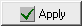
\includegraphics[height=0.5cm]{Settings_Ini_Apply.png} and then Save 
\includegraphics[height=0.5cm]{Settings_Ini_Save.png} button.
%HERE


\item After editing, insert the sample into the sensor head and activate the corresponding row by double-clicking on any row cell. Click the Run button 
\includegraphics[height=1cm]{Btn_Start.jpg}.
The following message will be shown. Otherwise, stop the application and check the mode switcher position.

\begin{figure}[H]
\centering
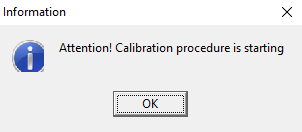
\includegraphics[width=6cm]{Calibration_notification.png}
\caption{Calibration notification}
\label{fig:Calibration_notification}
\end{figure}

\item Wait for the Done message to appear.

\begin{figure}[H]
\centering
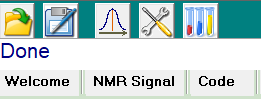
\includegraphics[width=5cm]{Calibration_Done.PNG}
\caption{The message in the end of the calibration}
\label{fig:Cal_Completed}
\end{figure}

Target values and coefficients will be calculated automatically, when the calibration is finished. 

\item Press the Apply 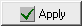
\includegraphics[height=0.5cm]{Settings_Ini_Apply.png} button to save changes.

\item Repeat previous calibration steps for other calibration samples.

\item Save the application with the new calibration data by pressing the Save button 
\includegraphics[width=0.5cm]{Btn_Save.png} in the main menu.
\end{enumerate}

\textbf{Attention!} Do not forget to switch the measurement mode after the calibration is done.

\subsection{Milk Powder}
\subsubsection{Protein content, Fat Content, Carbohydrate Content}

The application for measurement of protein content in mixture of Milk Powders is called
\texttt{Japan Demo milk powder protein}, for measurement of Fats content it is called \texttt{Japan Demo milk powder fat} application file and for carbohydrates content - \texttt{Japan Demo milk powder CH}. 

The essential parameters for these samples and applications are given in figures below.
Make sure that values of \texttt{Echo times},
\texttt{Relaxation period} and
\texttt{Amount of scans} are the same.

\begin{figure}[H]
\centering
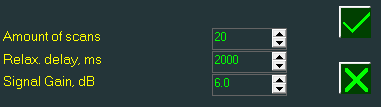
\includegraphics[width=10cm]{Gui_Milk_Fat.png}
\caption{Settings for protein content in milk powders application}
\label{fig:Gui Settings for protein content in milk powders application}
\end{figure}

\begin{figure}[H]
\centering
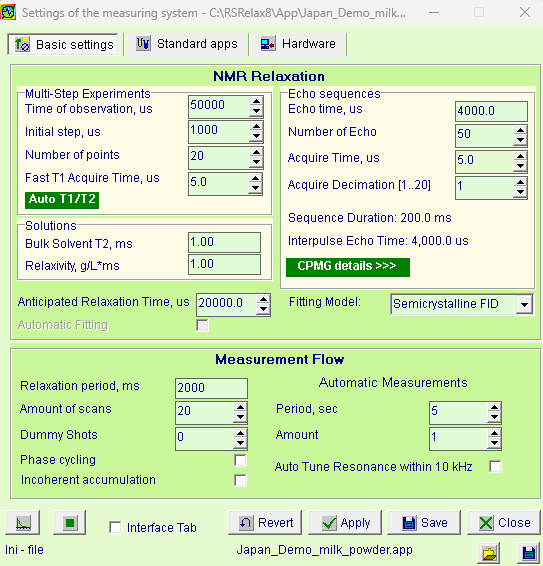
\includegraphics[width=10cm]{Settings_Milk_Fat.png}
\caption{Advanced settings for protein content in milk powders application}
\label{fig:Settings for protein content in milk powders application}
\end{figure}

In the figures below there are the calibration curves measured for the samples for protein content(\cref{fig:Calibration protein content in milk powders}), fat content (\cref{fig:Calibration fat content in milk powders}) and carbohydrates content (\cref{fig:Calibration CH content in milk powders}).

\begin{figure}[H]
\centering
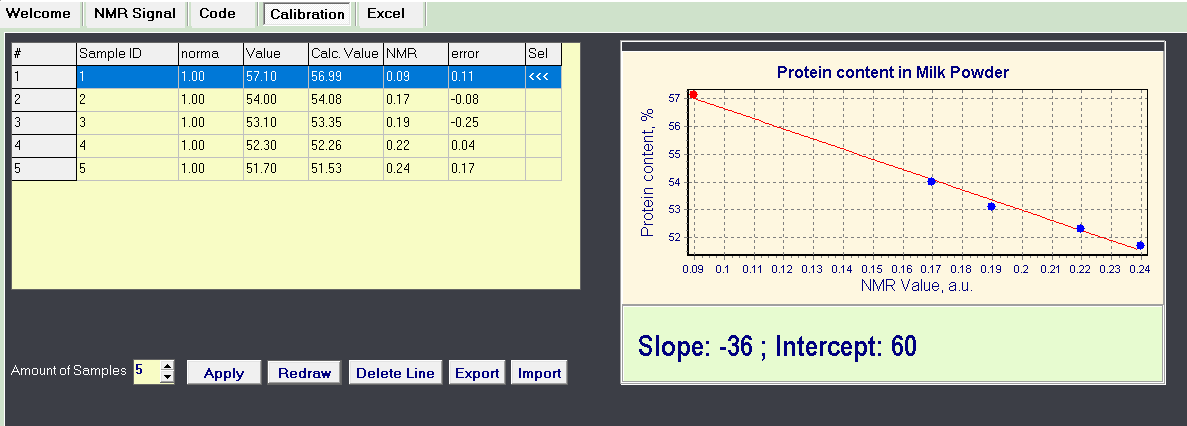
\includegraphics[width=17cm]{Calibration_Milk_Protein.png}
\caption{Calibration of the protein content in milk powders}
\label{fig:Calibration protein content in milk powders}
\end{figure}

\begin{figure}[H]
\centering
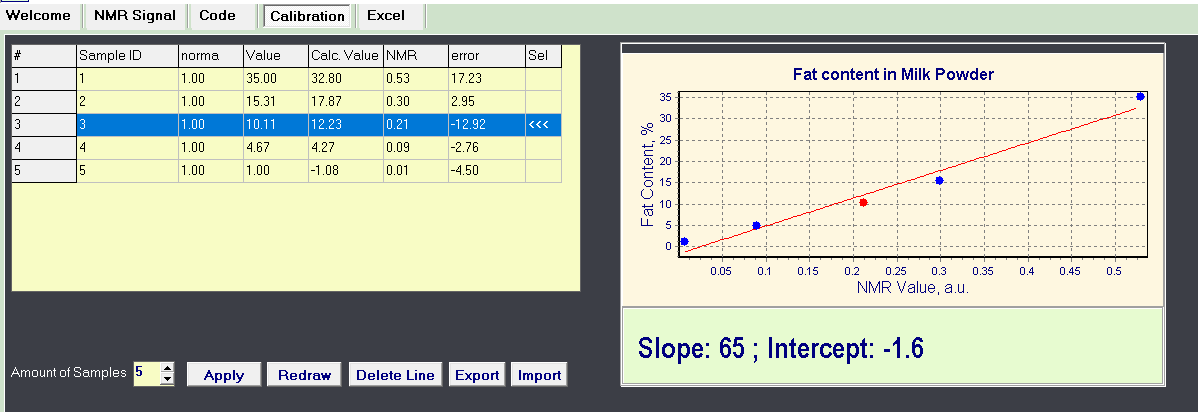
\includegraphics[width=17cm]{Calibration_Milk_Fat.png}
\caption{Calibration of the fat content in milk powders}
\label{fig:Calibration fat content in milk powders}
\end{figure}

\begin{figure}[H]
\centering
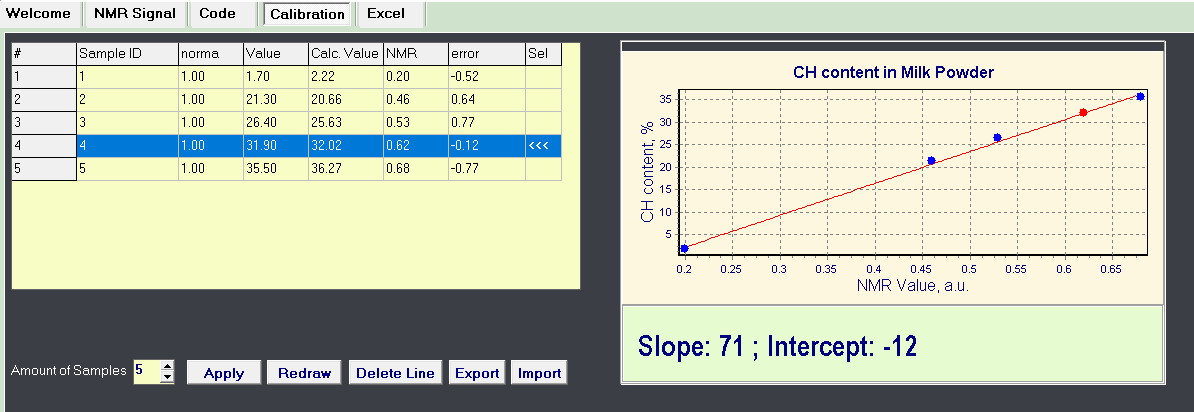
\includegraphics[width=17cm]{Calibration_Milk_CH.png}
\caption{Calibration of the C.H. content in milk powders}
\label{fig:Calibration CH content in milk powders}
\end{figure}

\textcolor{red}{\textbf{Attention!}} Do not forget to switch the measurement mode after the calibration is done.


\newpage
\subsection{Cookies}
\subsubsection{Fat Content, Carbohydrate Content}

The application for measurement of fat content in Cookies is called
\texttt{Japan Demo cookie fat},  and for carbohydrates content - \texttt{Japan Demo cookie CH}. 

Ensure that the values of \texttt{Echo times}, \texttt{Relaxation period}, \texttt{Amount of scans} are as given in the \cref{fig:Settings for protein content in cookie application} and \cref{fig:Gui Settings for protein content in cookie application}.

\begin{figure}[H]
\centering
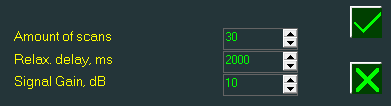
\includegraphics[width=10cm]{Gui_Cookie_Fat.png}
\caption{Settings for protein content in milk powders application}
\label{fig:Gui Settings for protein content in cookie application}
\end{figure}

\begin{figure}[H]
\centering
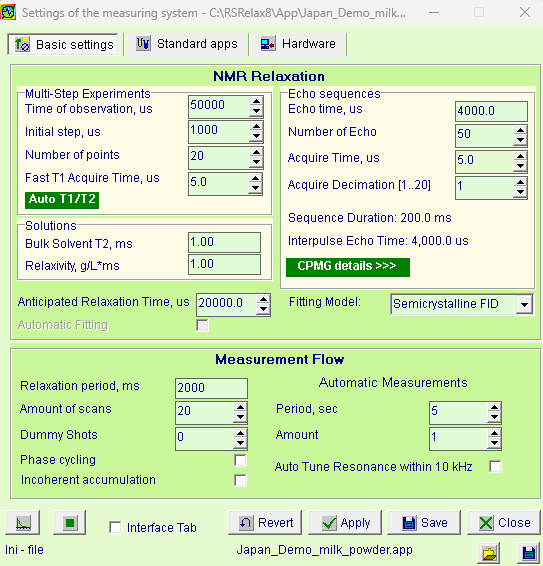
\includegraphics[width=10cm]{Settings_Milk_Fat.png}
\caption{Advanced settings for protein content in milk powders application}
\label{fig:Settings for protein content in cookie application}
\end{figure}

In the figures below there are the calibration curves measured for the samples for fat content (\cref{fig:Calibration fat content in cookies}) and carbohydrates content (\cref{fig:Calibration CH content in cookies}).

\begin{figure}[H]
\centering
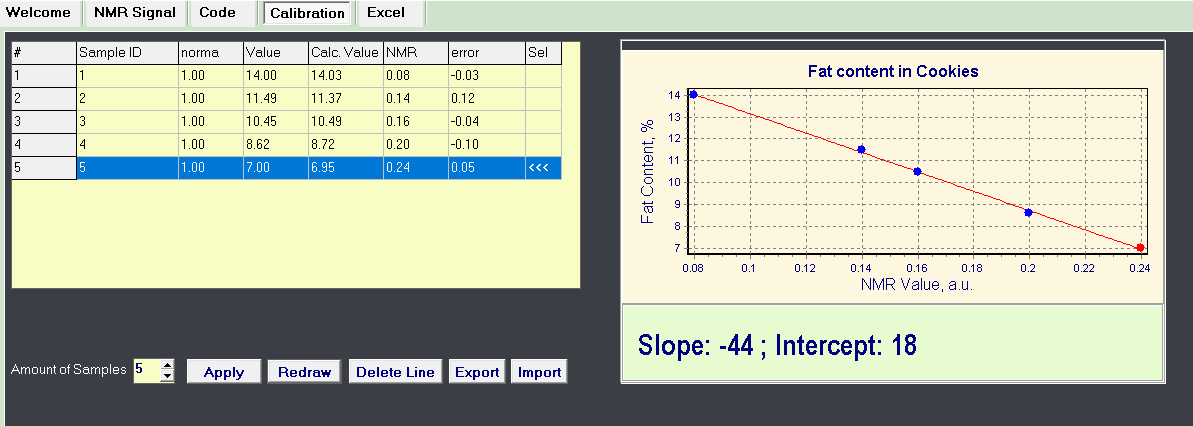
\includegraphics[width=17cm]{Calibration_Cook_Fat.png}
\caption{Calibration of the fat content in cookies}
\label{fig:Calibration fat content in cookies}
\end{figure}

\begin{figure}[H]
\centering
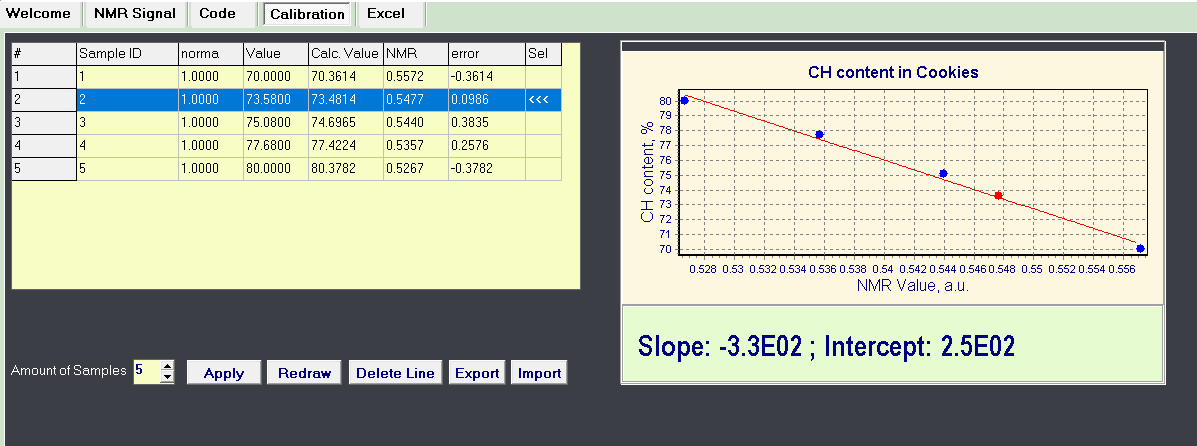
\includegraphics[width=17cm]{Calibration_Cookies_CH.png}
\caption{Calibration of the C.H. content in cookies}
\label{fig:Calibration CH content in cookies}
\end{figure}

\textcolor{red}{\textbf{Attention!}} Do not forget to switch the measurement mode after the calibration is done.

\newpage
\subsection{Butter}
\subsubsection{Fat content}


The application for measurement of fat content in butter is called
\texttt{Japan Demo butter}.


Ensure that the values of \texttt{Echo times}, \texttt{Relaxation period}, \texttt{Number of Echo}, \texttt{Acquire Time}, \texttt{Acquire Decimation} and \texttt{Amount of scans} are as given in the \cref{fig:Settings for CPMG} and 
make sure the same options are chosen in CPMG details as in \cref{fig:CPMG details}.

\begin{figure}[H]
\centering
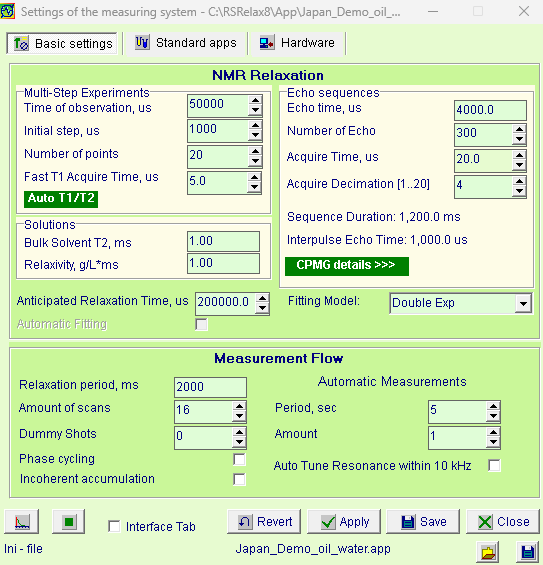
\includegraphics[width=10cm]{Settings_OilWater.png}
\caption{Settings for Fat content in butter application}
\label{fig:Settings for CPMG}
\end{figure}

\begin{figure}[H]
\centering
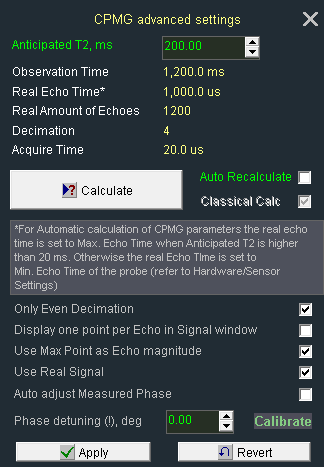
\includegraphics[width=7cm]{CPMG_Oil_Water.png}
\caption{Settings for CPMG details for Fat content in butter application}
\label{fig:CPMG details}
\end{figure}

In the figure below there is the calibration curve measured for the butter samples for fat content (\cref{fig:Calibration fat content in butter}).

\begin{figure}[H]
\centering
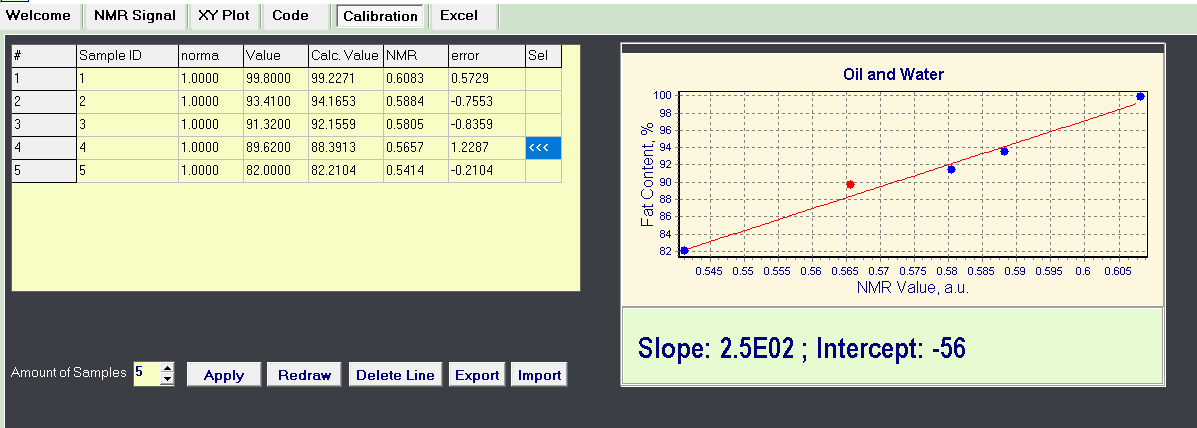
\includegraphics[width=17cm]{Calibration_Oil_water.png}
\caption{Calibration of the fat content in butter}
\label{fig:Calibration fat content in butter}
\end{figure}

\textcolor{red}{\textbf{Attention!}} Do not forget to switch the measurement mode after the calibration is done.

%Here



\newpage
\section{Measurement}
\label{sec:Measurement}

\begin{enumerate}[ref={observation~\arabic*}]

\item Press the Load application and Settings button 
\includegraphics[height=0.5cm]{Btn_Open.png} in the main menu to open the target application file. 

\item Ensure the device is in measurement mode:

\begin{figure}[H]
\centering
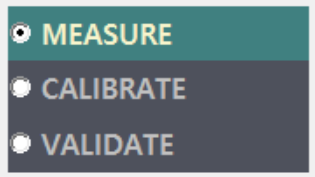
\includegraphics[width=4cm]{ModeSwitcher.png}
\caption{Measurement mode}
\label{fig:Mode Switcher2}
\end{figure}


\item Insert the corresponding sample into the sensor probe head.

\item Enter sample name by clicking on Sample Info Panel button 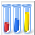
\includegraphics[height=0.5cm]{Btn_Sample.png}.

\begin{figure}[!ht]
\centering
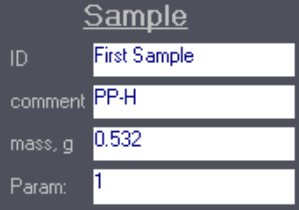
\includegraphics[width=4cm]{Sample_parameters.PNG}
\caption{Set sample parameters}
\label{fig:Set sample parameters}
\end{figure}

\item Save changes by clicking on Apply All button 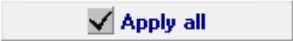
\includegraphics[height=0.4cm]{Sample_Apply.png} on the Sample Info panel.

\item Ensure the necessary parameters for each application correspond to those listed in the Calibration steps.

\item Press the run button 
\includegraphics[height=1cm]{Btn_Start.jpg} to start the measurement.

\item Wait for result of the measurement to appear in the Excel Tab:

\begin{figure}[H]
\centering
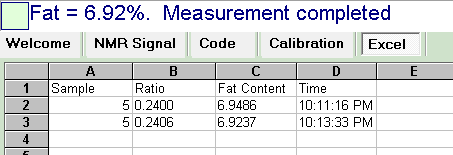
\includegraphics[width=10cm]{Measurement_Cookie_Fat.png}
\caption{The result of the measurement in the Excel Tab}
\label{fig:Measurement_Completed}
\end{figure}

\end{enumerate}

\end{document}
